\documentclass[tikz,crop]{standalone}
\usepackage{tikz}
\usepackage{pgfplots}
\pgfplotsset{compat=1.18}

\begin{document}
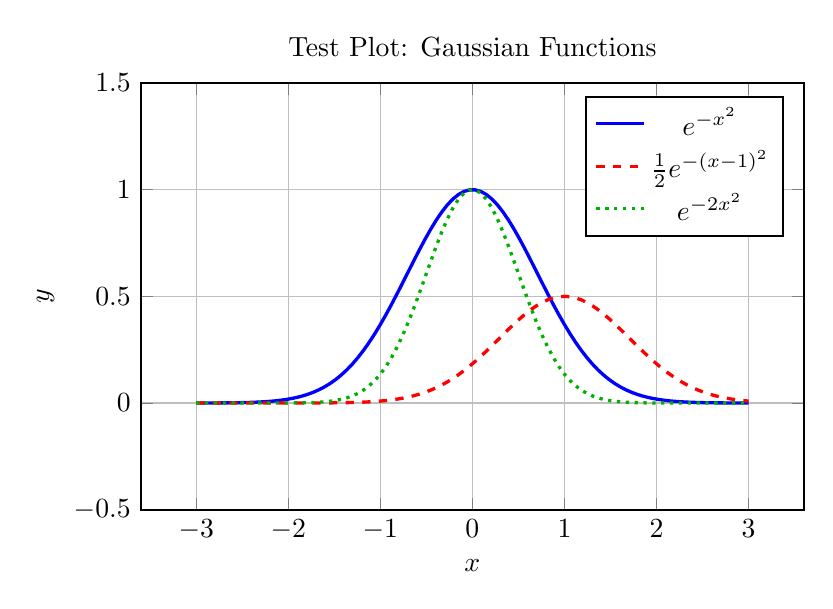
\begin{tikzpicture}
  \begin{axis}[
    width=10cm, height=7cm,
    xlabel={$x$},
    ylabel={$y$},
    title={Test Plot: Gaussian Functions},
    grid=both,
    thick,
    samples=100,
    domain=-3:3,
    ymin=-0.5, ymax=1.5,
    legend pos=north east
  ]
    \addplot[blue, very thick] {exp(-x^2)};
    \addlegendentry{$e^{-x^2}$}

    \addplot[red, very thick, dashed] {0.5*exp(-(x-1)^2)};
    \addlegendentry{$\frac{1}{2}e^{-(x-1)^2}$}

    \addplot[green!70!black, very thick, dotted] {exp(-2*x^2)};
    \addlegendentry{$e^{-2x^2}$}
  \end{axis}
\end{tikzpicture}
\end{document}
